\documentclass[doc]{apa6}\usepackage[]{graphicx}\usepackage[]{color}
%% maxwidth is the original width if it is less than linewidth
%% otherwise use linewidth (to make sure the graphics do not exceed the margin)
\makeatletter
\def\maxwidth{ %
  \ifdim\Gin@nat@width>\linewidth
    \linewidth
  \else
    \Gin@nat@width
  \fi
}
\makeatother

\definecolor{fgcolor}{rgb}{0.345, 0.345, 0.345}
\newcommand{\hlnum}[1]{\textcolor[rgb]{0.686,0.059,0.569}{#1}}%
\newcommand{\hlstr}[1]{\textcolor[rgb]{0.192,0.494,0.8}{#1}}%
\newcommand{\hlcom}[1]{\textcolor[rgb]{0.678,0.584,0.686}{\textit{#1}}}%
\newcommand{\hlopt}[1]{\textcolor[rgb]{0,0,0}{#1}}%
\newcommand{\hlstd}[1]{\textcolor[rgb]{0.345,0.345,0.345}{#1}}%
\newcommand{\hlkwa}[1]{\textcolor[rgb]{0.161,0.373,0.58}{\textbf{#1}}}%
\newcommand{\hlkwb}[1]{\textcolor[rgb]{0.69,0.353,0.396}{#1}}%
\newcommand{\hlkwc}[1]{\textcolor[rgb]{0.333,0.667,0.333}{#1}}%
\newcommand{\hlkwd}[1]{\textcolor[rgb]{0.737,0.353,0.396}{\textbf{#1}}}%

\usepackage{framed}
\makeatletter
\newenvironment{kframe}{%
 \def\at@end@of@kframe{}%
 \ifinner\ifhmode%
  \def\at@end@of@kframe{\end{minipage}}%
  \begin{minipage}{\columnwidth}%
 \fi\fi%
 \def\FrameCommand##1{\hskip\@totalleftmargin \hskip-\fboxsep
 \colorbox{shadecolor}{##1}\hskip-\fboxsep
     % There is no \\@totalrightmargin, so:
     \hskip-\linewidth \hskip-\@totalleftmargin \hskip\columnwidth}%
 \MakeFramed {\advance\hsize-\width
   \@totalleftmargin\z@ \linewidth\hsize
   \@setminipage}}%
 {\par\unskip\endMakeFramed%
 \at@end@of@kframe}
\makeatother

\definecolor{shadecolor}{rgb}{.97, .97, .97}
\definecolor{messagecolor}{rgb}{0, 0, 0}
\definecolor{warningcolor}{rgb}{1, 0, 1}
\definecolor{errorcolor}{rgb}{1, 0, 0}
\newenvironment{knitrout}{}{} % an empty environment to be redefined in TeX

\usepackage{alltt}
\usepackage{longtable} % needed for reporttools tables.
\usepackage{pdflscape} % for landscape pages.
\usepackage{hyperref}  % package used for hyperlinked toc.
\usepackage [toc, page]{appendix} % used for appendices
\usepackage{verbatim}
\IfFileExists{upquote.sty}{\usepackage{upquote}}{}


\begin{document}

\author{William Murrah}
\title{STAR Example Intent-to-treat Report}
\maketitle
\tableofcontents







\clearpage
\section{Introduction}

This is an example report of the \emph{STAR} data. The data consists of 150 cases and 11 variables. This example is a simplified version of the types of internal lab reports that can be generated using R and the \texttt{knitr} package to produce reproducible analyses. 

\clearpage
\begin{landscape}
\section{Descriptive Statistics}

\begin{tabular}{llccccc}
\hline
& & \multicolumn{4}{c}{schoolk} & \multicolumn{1}{c}{} \\ 
 &  & inner-city & rural & suburban & urban & \multicolumn{1}{c}{All} \\ 
\hline
mathk & Mean  & $460.00$ & $484.50$ & $492.23$ & $502.85$ & $483.28$ \\
 & SD  & $\phantom{0}56.80$ & $\phantom{0}46.34$ & $\phantom{0}44.82$ & $\phantom{0}46.16$ & $\phantom{0}49.25$ \\
readk & Mean  & $422.48$ & $438.21$ & $445.47$ & $432.69$ & $436.39$ \\
 & SD  & $\phantom{0}23.69$ & $\phantom{0}30.67$ & $\phantom{0}36.96$ & $\phantom{0}20.20$ & $\phantom{0}30.88$ \\
\hline 
\end{tabular}


\clearpage
% latex table generated in R 3.1.0 by xtable 1.7-3 package
% Sun Apr 13 12:19:33 2014
{\footnotesize
\begin{longtable}{ll|rrr|rrr|rrr|rrr}
 \textbf{Variable} & \textbf{Levels} & $\mathbf{n_{\mathrm{regular}}}$ & $\mathbf{\%_{\mathrm{regular}}}$ & $\mathbf{\sum \%_{\mathrm{regular}}}$ & $\mathbf{n_{\mathrm{regular+aide}}}$ & $\mathbf{\%_{\mathrm{regular+aide}}}$ & $\mathbf{\sum \%_{\mathrm{regular+aide}}}$ & $\mathbf{n_{\mathrm{small}}}$ & $\mathbf{\%_{\mathrm{small}}}$ & $\mathbf{\sum \%_{\mathrm{small}}}$ & $\mathbf{n_{\mathrm{all}}}$ & $\mathbf{\%_{\mathrm{all}}}$ & $\mathbf{\sum \%_{\mathrm{all}}}$ \\ 
  \hline
gender & female & 25 & 49.0 & 49.0 & 30 & 54.5 & 54.5 & 21 & 47.7 & 47.7 & 76 & 50.7 & 50.7 \\ 
   & male & 26 & 51.0 & 100.0 & 25 & 45.5 & 100.0 & 23 & 52.3 & 100.0 & 74 & 49.3 & 100.0 \\ 
   \hline
$p= 0.76$ & all & 51 & 100.0 &  & 55 & 100.0 &  & 44 & 100.0 &  & 150 & 100.0 &  \\ 
   \hline
\hline
ethnicity & afam & 15 & 29.4 & 29.4 & 12 & 21.8 & 21.8 & 12 & 27.3 & 27.3 & 39 & 26.0 & 26.0 \\ 
   & cauc & 36 & 70.6 & 100.0 & 43 & 78.2 & 100.0 & 32 & 72.7 & 100.0 & 111 & 74.0 & 100.0 \\ 
   \hline
$p= 0.66$ & all & 51 & 100.0 &  & 55 & 100.0 &  & 44 & 100.0 &  & 150 & 100.0 &  \\ 
   \hline
\hline
schoolk & inner-city & 12 & 23.5 & 23.5 & 8 & 14.6 & 14.6 & 9 & 20.4 & 20.4 & 29 & 19.3 & 19.3 \\ 
   & rural & 27 & 52.9 & 76.5 & 28 & 50.9 & 65.5 & 17 & 38.6 & 59.1 & 72 & 48.0 & 67.3 \\ 
   & suburban & 8 & 15.7 & 92.2 & 12 & 21.8 & 87.3 & 14 & 31.8 & 90.9 & 34 & 22.7 & 90.0 \\ 
   & urban & 4 & 7.8 & 100.0 & 7 & 12.7 & 100.0 & 4 & 9.1 & 100.0 & 15 & 10.0 & 100.0 \\ 
   \hline
$p= 0.45$ & all & 51 & 100.0 &  & 55 & 100.0 &  & 44 & 100.0 &  & 150 & 100.0 &  \\ 
   \hline
\hline
birth & 1978 Q4 & 0 & 0.0 & 0.0 & 1 & 1.8 & 1.8 & 0 & 0.0 & 0.0 & 1 & 0.7 & 0.7 \\ 
   & 1979 Q1 & 0 & 0.0 & 0.0 & 0 & 0.0 & 1.8 & 1 & 2.3 & 2.3 & 1 & 0.7 & 1.3 \\ 
   & 1979 Q2 & 2 & 3.9 & 3.9 & 0 & 0.0 & 1.8 & 0 & 0.0 & 2.3 & 2 & 1.3 & 2.7 \\ 
   & 1979 Q3 & 0 & 0.0 & 3.9 & 0 & 0.0 & 1.8 & 2 & 4.5 & 6.8 & 2 & 1.3 & 4.0 \\ 
   & 1979 Q4 & 6 & 11.8 & 15.7 & 15 & 27.3 & 29.1 & 5 & 11.4 & 18.2 & 26 & 17.3 & 21.3 \\ 
   & 1980 Q1 & 13 & 25.5 & 41.2 & 11 & 20.0 & 49.1 & 9 & 20.4 & 38.6 & 33 & 22.0 & 43.3 \\ 
   & 1980 Q2 & 15 & 29.4 & 70.6 & 16 & 29.1 & 78.2 & 13 & 29.6 & 68.2 & 44 & 29.3 & 72.7 \\ 
   & 1980 Q3 & 15 & 29.4 & 100.0 & 12 & 21.8 & 100.0 & 14 & 31.8 & 100.0 & 41 & 27.3 & 100.0 \\ 
   \hline
$p= 0.16$ & all & 51 & 100.0 &  & 55 & 100.0 &  & 44 & 100.0 &  & 150 & 100.0 &  \\ 
   \hline
\hline
lunchk & free & 29 & 56.9 & 56.9 & 22 & 40.7 & 40.7 & 12 & 27.9 & 27.9 & 63 & 42.6 & 42.6 \\ 
   & non-free & 22 & 43.1 & 100.0 & 32 & 59.3 & 100.0 & 31 & 72.1 & 100.0 & 85 & 57.4 & 100.0 \\ 
   \hline
$p= 0.02$ & all & 51 & 100.0 &  & 54 & 100.0 &  & 43 & 100.0 &  & 148 & 100.0 &  \\ 
   \hline
\hline
\hline
\caption{Descriptive Statistics for Qualitative Variables} 
\label{}
\end{longtable}
}


\clearpage
% latex table generated in R 3.1.0 by xtable 1.7-3 package
% Sun Apr 13 12:19:33 2014
{\footnotesize
\begin{longtable}{llrrrrrrrrrr}
 \textbf{Variable} & \textbf{Levels} & $\mathbf{n}$ & \textbf{Min} & $\mathbf{q_1}$ & $\mathbf{\widetilde{x}}$ & $\mathbf{\bar{x}}$ & $\mathbf{q_3}$ & \textbf{Max} & $\mathbf{s}$ & \textbf{IQR} & \textbf{\#NA} \\ 
  \hline
readk & regular &  44 & 360 & 410.8 & 432.0 & 433.6 & 453.5 & 507 & 30.3 & 42.8 &  7 \\ 
   & regular+aide &  52 & 388 & 413.0 & 433.0 & 438.3 & 458.5 & 580 & 35.4 & 45.5 &  3 \\ 
   & small &  40 & 397 & 421.8 & 436.0 & 437.0 & 447.0 & 527 & 25.3 & 25.2 &  4 \\ 
   \hline
$p= 0.75$ & all & 136 & 360 & 414.0 & 433.0 & 436.4 & 451.0 & 580 & 30.9 & 37.0 & 14 \\ 
   \hline
read1 & regular &  30 & 434 & 477.2 & 504.0 & 517.7 & 543.0 & 651 & 58.5 & 65.8 & 21 \\ 
   & regular+aide &  38 & 436 & 489.0 & 528.5 & 530.4 & 562.5 & 651 & 56.7 & 73.5 & 17 \\ 
   & small &  29 & 430 & 482.0 & 516.0 & 522.4 & 553.0 & 651 & 55.5 & 71.0 & 15 \\ 
   \hline
$p= 0.65$ & all &  97 & 430 & 478.0 & 516.0 & 524.1 & 558.0 & 651 & 56.6 & 80.0 & 53 \\ 
   \hline
mathk & regular &  45 & 320 & 439.0 & 468.0 & 475.9 & 506.0 & 602 & 54.3 & 67.0 &  6 \\ 
   & regular+aide &  52 & 392 & 449.0 & 473.0 & 482.4 & 509.5 & 626 & 48.8 & 60.5 &  3 \\ 
   & small &  40 & 412 & 463.0 & 489.0 & 492.8 & 514.8 & 626 & 43.3 & 51.8 &  4 \\ 
   \hline
$p= 0.29$ & all & 137 & 320 & 449.0 & 478.0 & 483.3 & 513.0 & 626 & 49.3 & 64.0 & 13 \\ 
   \hline
math1 & regular &  30 & 444 & 495.5 & 533.5 & 534.6 & 562.0 & 653 & 48.1 & 66.5 & 21 \\ 
   & regular+aide &  41 & 444 & 502.0 & 529.0 & 535.0 & 562.0 & 627 & 42.7 & 60.0 & 14 \\ 
   & small &  30 & 441 & 497.8 & 521.5 & 530.2 & 569.8 & 627 & 49.4 & 72.0 & 14 \\ 
   \hline
$p= 0.90$ & all & 101 & 441 & 500.0 & 529.0 & 533.5 & 562.0 & 653 & 46.0 & 62.0 & 49 \\ 
   \hline
\hline
\caption{Descriptive Statistics for Qauntitative Variables} 
\label{}
\end{longtable}
}


\end{landscape}
\clearpage

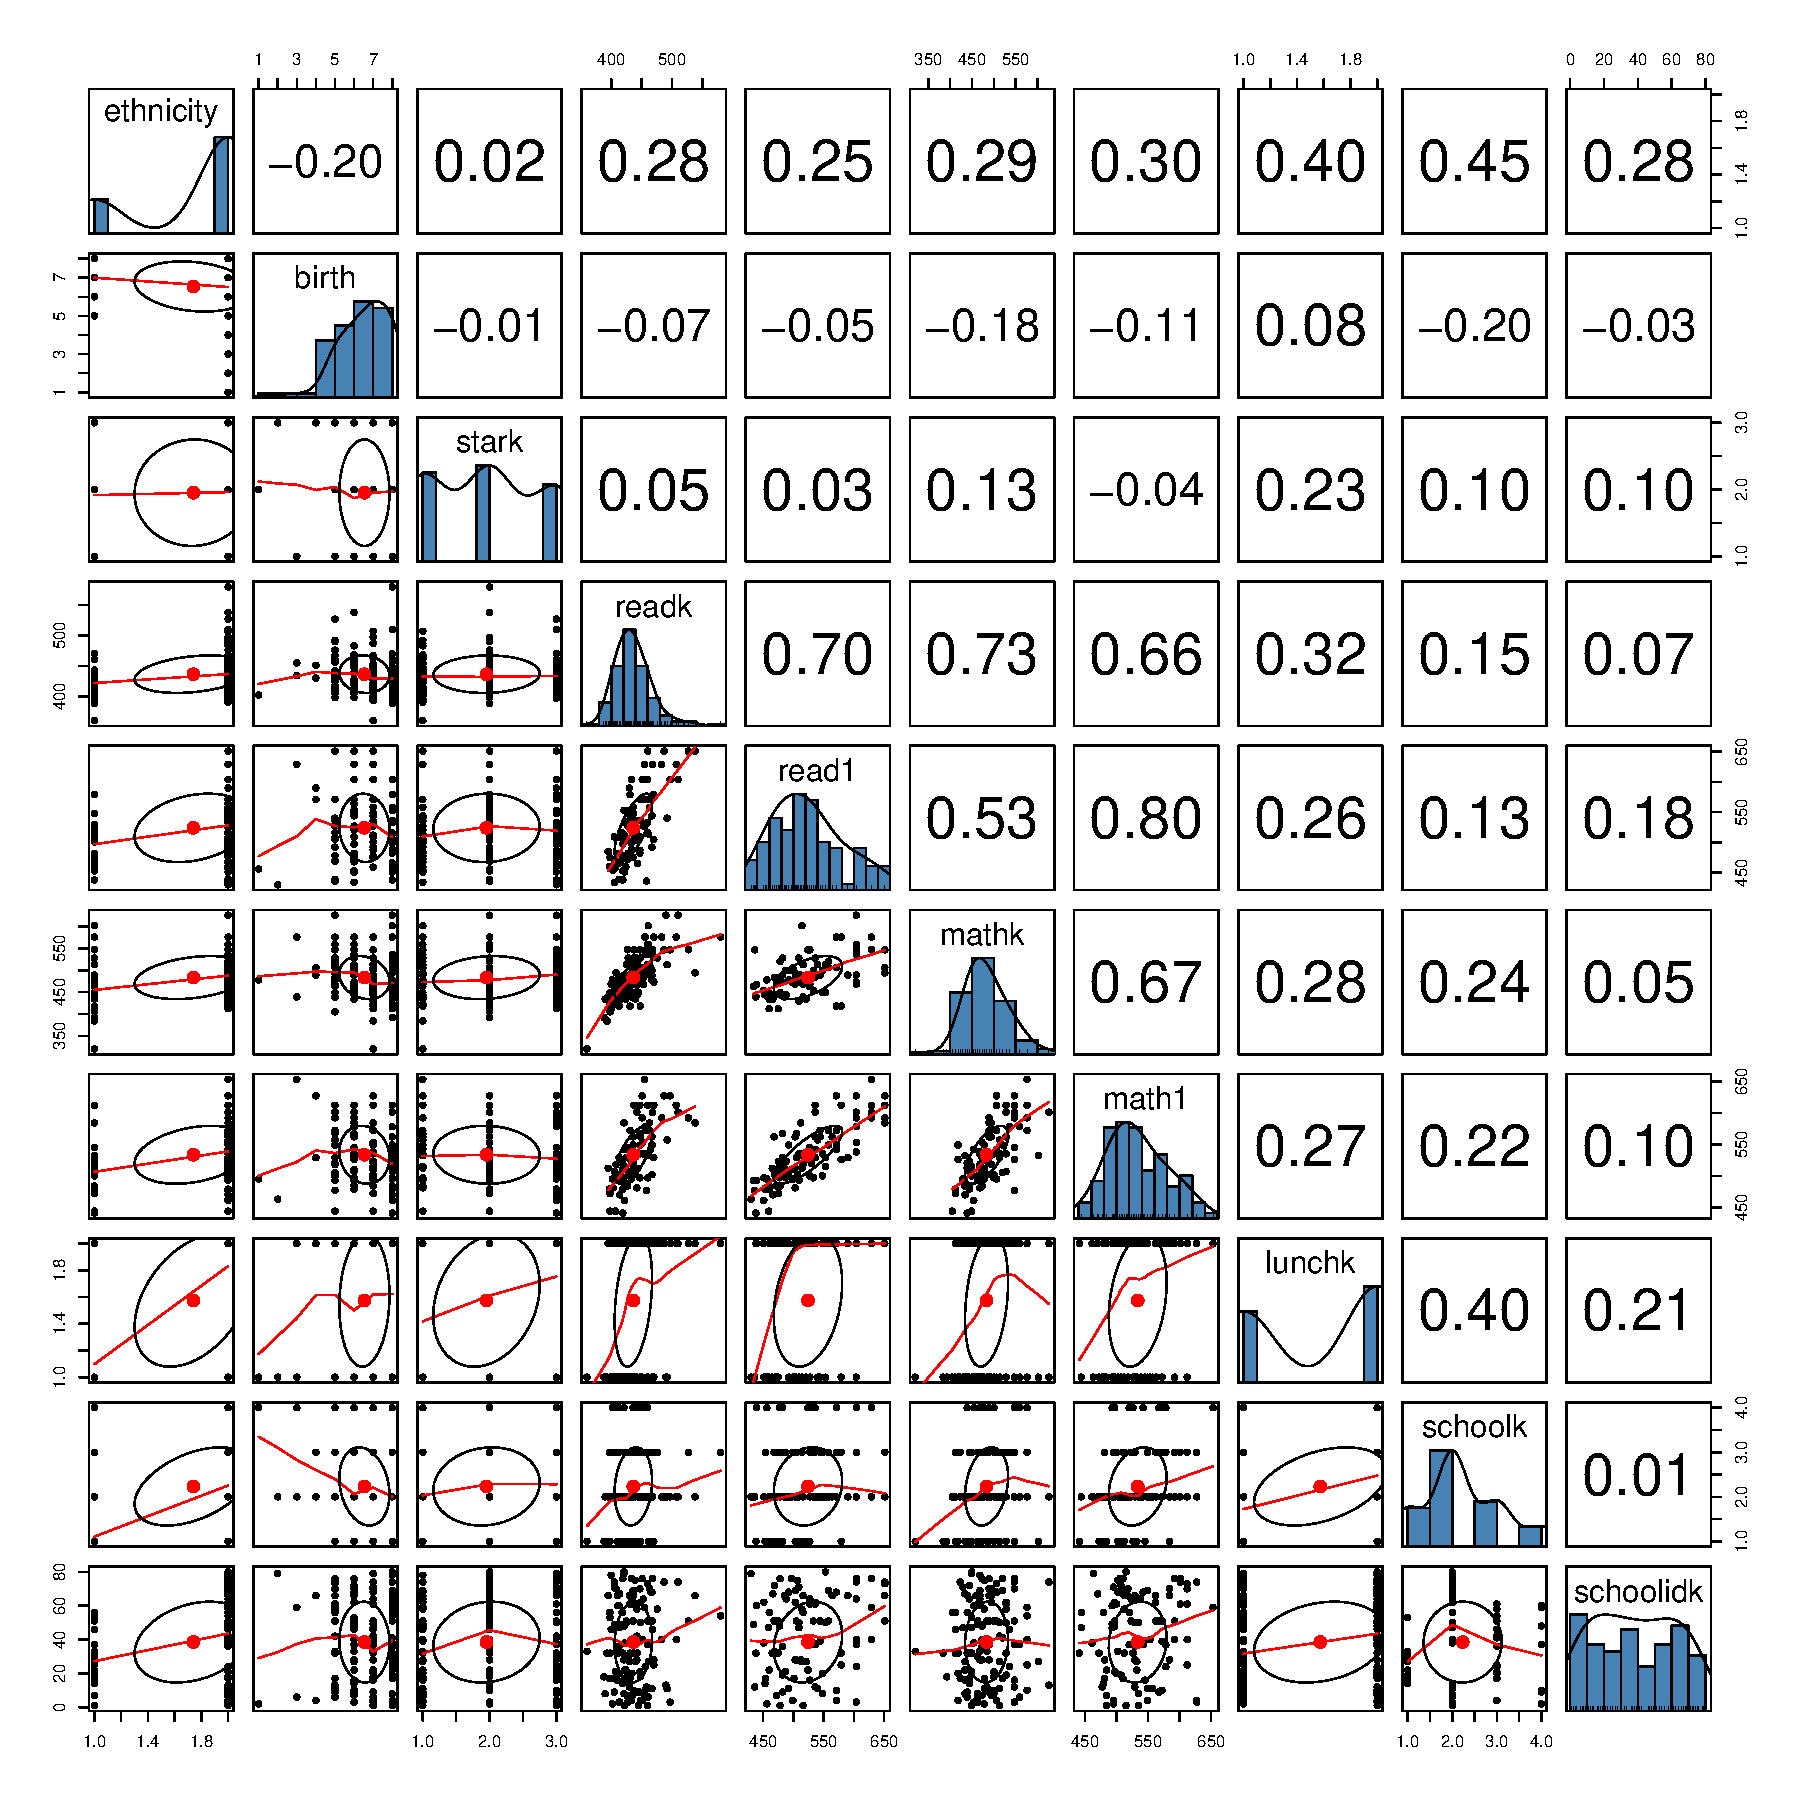
\includegraphics[width=\maxwidth]{figure/pairsplot} 


\clearpage
\section{Intent-to-treat Analyses}
\subsection{Pretest-posttest Regressions}

\begin{table}[h]
\begin{center}
\begin{tabular}{l c c }
\hline
                  & Reading & Math \\
\hline
(Intercept)       & $-97.99$     & $197.05^{***}$ \\
                  & $(73.34)$    & $(40.81)$      \\
starkregular+aide & $7.88$       & $2.12$         \\
                  & $(10.93)$    & $(8.82)$       \\
starksmall        & $6.88$       & $-10.43$       \\
                  & $(12.57)$    & $(10.08)$      \\
pretest           & $1.36^{***}$ & $0.65^{***}$   \\
                  & $(0.17)$     & $(0.08)$       \\
gendermale        & $-1.06$      & $12.29$        \\
                  & $(9.35)$     & $(7.49)$       \\
ethnicitycauc     & $8.30$       & $18.83$        \\
                  & $(18.51)$    & $(14.17)$      \\
lunchknon-free    & $6.66$       & $11.63$        \\
                  & $(11.50)$    & $(8.91)$       \\
schoolkrural      & $13.07$      & $-7.93$        \\
                  & $(21.85)$    & $(16.74)$      \\
schoolksuburban   & $10.92$      & $4.29$         \\
                  & $(20.26)$    & $(16.05)$      \\
schoolkurban      & $11.78$      & $-20.67$       \\
                  & $(24.62)$    & $(19.47)$      \\
\hline
R$^2$             & 0.52         & 0.51           \\
Adj. R$^2$        & 0.46         & 0.46           \\
Num. obs.         & 88           & 92             \\
\hline
\multicolumn{3}{l}{\scriptsize{$^{***}p<0.001$, $^{**}p<0.01$, $^*p<0.05$}}
\end{tabular}
\caption{Unstandardized ITT Models}
\label{table:coefficients}
\end{center}
\end{table}





\begin{table}[h]
\begin{center}
\begin{tabular}{l c c }
\hline
                  & Reading & Math \\
\hline
(Intercept)       & $-0.53^{*}$  & $-0.52^{*}$  \\
                  & $(0.25)$     & $(0.26)$     \\
starkregular+aide & $0.14$       & $0.05$       \\
                  & $(0.19)$     & $(0.19)$     \\
starksmall        & $0.12$       & $-0.23$      \\
                  & $(0.22)$     & $(0.22)$     \\
scale(pretest)    & $0.74^{***}$ & $0.69^{***}$ \\
                  & $(0.09)$     & $(0.09)$     \\
gendermale        & $-0.02$      & $0.27$       \\
                  & $(0.17)$     & $(0.16)$     \\
ethnicitycauc     & $0.15$       & $0.41$       \\
                  & $(0.33)$     & $(0.31)$     \\
lunchknon-free    & $0.12$       & $0.25$       \\
                  & $(0.20)$     & $(0.19)$     \\
schoolkrural      & $0.23$       & $-0.17$      \\
                  & $(0.39)$     & $(0.36)$     \\
schoolksuburban   & $0.19$       & $0.09$       \\
                  & $(0.36)$     & $(0.35)$     \\
schoolkurban      & $0.21$       & $-0.45$      \\
                  & $(0.44)$     & $(0.42)$     \\
\hline
R$^2$             & 0.52         & 0.51         \\
Adj. R$^2$        & 0.46         & 0.46         \\
Num. obs.         & 88           & 92           \\
\hline
\multicolumn{3}{l}{\scriptsize{$^{***}p<0.001$, $^{**}p<0.01$, $^*p<0.05$}}
\end{tabular}
\caption{Standardized ITT Models}
\label{table:coefficients}
\end{center}
\end{table}



\clearpage
\clearpage
\begin{appendices}
\section{Data Preparation Code}
\label{rcode}
\subsection{starRmake.R}
\verbatiminput{../../../data/starRmake.R}
\subsection{prePost.R}
\verbatiminput{../../../analyses/prePost.R}
\subsection{stdPrePost.R}
\verbatiminput{../../../analyses/stdPrePost.R}
\clearpage
\section{R Session Information}
\begin{knitrout}
\definecolor{shadecolor}{rgb}{0.969, 0.969, 0.969}\color{fgcolor}\begin{kframe}
\begin{verbatim}
R version 3.1.0 (2014-04-10)
Platform: x86_64-pc-linux-gnu (64-bit)

locale:
 [1] LC_CTYPE=en_US.UTF-8       LC_NUMERIC=C              
 [3] LC_TIME=en_US.UTF-8        LC_COLLATE=en_US.UTF-8    
 [5] LC_MONETARY=en_US.UTF-8    LC_MESSAGES=en_US.UTF-8   
 [7] LC_PAPER=en_US.UTF-8       LC_NAME=C                 
 [9] LC_ADDRESS=C               LC_TELEPHONE=C            
[11] LC_MEASUREMENT=en_US.UTF-8 LC_IDENTIFICATION=C       

attached base packages:
 [1] tcltk     splines   grid      stats     graphics  grDevices utils    
 [8] datasets  methods   base     

other attached packages:
 [1] texreg_1.31          reporttools_1.1.1    xtable_1.7-3        
 [4] VIMGUI_0.9.0         gWidgetsRGtk2_0.0-82 gWidgets_0.0-52     
 [7] RGtk2_2.20.27        survey_3.29-5        VIM_4.0.0           
[10] colorspace_1.2-4     tkrplot_0.0-23       tables_0.7.64       
[13] Hmisc_3.14-3         Formula_1.1-1        survival_2.37-7     
[16] lattice_0.20-29      psych_1.4.3          knitr_1.5           

loaded via a namespace (and not attached):
 [1] Cairo_1.5-5         car_2.0-19          class_7.3-10       
 [4] cluster_1.15.2      DEoptimR_1.0-1      e1071_1.6-3        
 [7] evaluate_0.5.3      foreign_0.8-61      formatR_0.10       
[10] glmnet_1.9-5        latticeExtra_0.6-26 MASS_7.3-31        
[13] Matrix_1.1-3        nnet_7.3-8          RColorBrewer_1.0-5 
[16] Rcpp_0.11.1         robustbase_0.90-2   sp_1.0-15          
[19] stringr_0.6.2       tools_3.1.0         vcd_1.3-1          
\end{verbatim}
\end{kframe}
\end{knitrout}

\end{appendices}
\end{document}
